\section{Methods}
\subsection{Study Design}
We constructed a deterministic compartmental model of \MPXV transmission.
Although stochastic network-based models can capture
uncertainty and complex contact patterns better,
deterministic compartmental models can estimate expected epidemic dynamics
and have smaller data requirements,
which are attractive during an emerging epidemic \cite{Johnson2016}.
Risk heterogeneity and associated mixing patterns can also be captured in
compartmental models via risk-based population stratification \cite{Garnett1996}.
\subsection{Setting \& Population}
The modelled population represents
2 partially connected sexual transmission networks of \GBMSM,
although the model captures both sexual and nonsexual transmission.
For the purposes of this study, we interpreted the two networks as two cities (cities A, B),
having a combined \GBMSM community size of 100,000 people.
\par
To ground our analyses in a plausible epidemic context in Canada,
we used the early \MPXV situation in Ontario.
The first reported case in Ontario occurred 2023 May 20 \cite{PHO2022ont};
therefore, we posited possible exposures up to 21 days before in Toronto.
Pre-exposure prophylaxis vaccination began 2022 June 12 \cite{TPH2022}.
At the time of initial vaccination rollout, about 5000 doses were available in Ontario
and decisions were underway about optimal allocation of this limited supply
across health units and cities in the province \cite{Mishra2022}.
\subsection{Model structure \& Parameterization}
Our model included 6 health states:
susceptible, vaccinated, exposed, infectious, isolating, and recovered
(Figure~\ref{fig:model.health}).
Each city was further stratified by levels of sexual risk
(higher or lower, defined by the numbers of sexual partners)
to reflect vaccine prioritization \cite{NACI2022vax}
and observed differences in the risk of \MPXV infectionc \cite{WHO2022}
(Figure~\ref{fig:model.city.risk}).
The definitions of higher and lower levels of sexual risk are outlined in Appendix~\ref{app.model}.
\par
To parameterize the model, we drew on
previous analyses of \GBMSM sexual networks in Canada \cite{Wang2021,Armstrong2020},
and emerging \MPXV epidemiological data in the context of the current epidemic
\cite{PHO2022synth,Adler2022,Thornhill2022,Charniga2022,Miura2022}.
We calibrated the average numbers of sexal partners among the higher-risk group
to obtain city-specific $R_0$ that ranged from 1 to 2.
Appendix~\ref{app.model} provides additional details about
the model implementation and parameterization.
\par
\begin{figure}
  \begin{subfigure}[b]{0.49\linewidth}
    \centerline{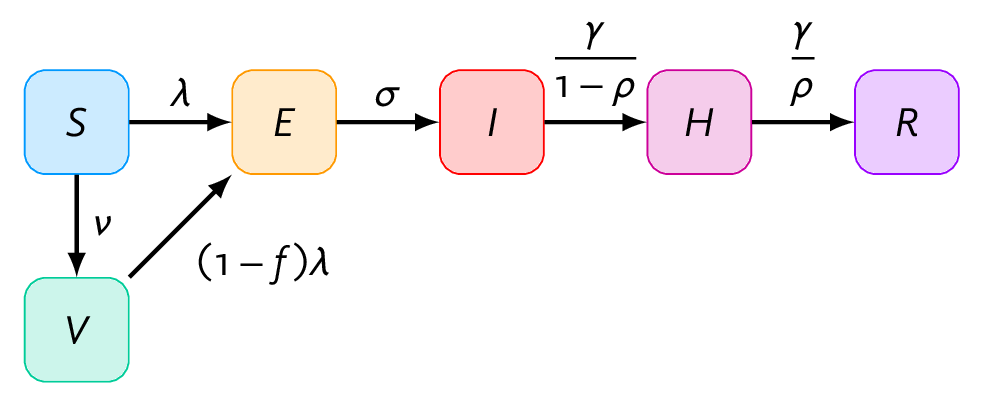
\includegraphics[scale=.8]{model.health}}
    \vskip3em
    \caption{Health states and transitions}
    \label{fig:model.health}
  \end{subfigure}\hfill
  \begin{subfigure}[b]{0.49\linewidth}
    \centerline{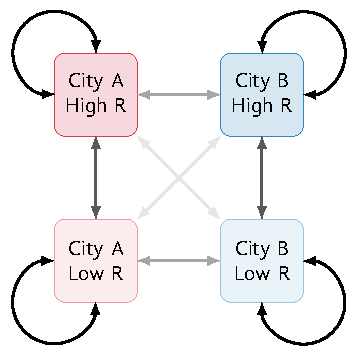
\includegraphics[scale=.8]{model.city.risk}}
    \caption{Cities, risk groups, and contact networks}
    \label{fig:model.city.risk}
  \end{subfigure}
  \caption{Model structure}
  \label{fig:model}
  \floatfoot
  (\subref{fig:model.city.risk})
  High/Low R: risk groups;
  arrow opacity is proportional to contact network connectivity between groups.
  (\subref{fig:model.health})
  $S$:~susceptible;
  $V$:~vaccinated;
  $E$:~exposed;
  $I$:~infectious;
  $R$:~recovered.
  See Table~\ref{tab:notation} and Appendix~\ref{app.model} for rate definitions.
\end{figure}
\begin{table}
  \caption{Model parameters, including default values and ranges explored via grid sweep}
  \label{tab:model.params}
  \small
\begin{tabular}{llrcc}
  \toprule
  Parameter                          & Stratum                   &      Value &      Range       & Ref \\
  \midrule
  Population size                    & overall                   &    100,000 &                  & \cite{Wang2021}\tn{a} \\
                                     & fraction in city A        &        .50 &    [.20,~.80]    & \tn{a} \\
  Fraction higher risk               & city A                    &        .10 & [.01,~.50]\tn{b} & \cite{Wang2021}\tn{a} \\
                                     & city B                    &        .10 &                  & \cite{Wang2021}\tn{a} \\[1ex]
  Contact rate                       & close non-sexual, all     &          1 &                  & \tn{a} \\
                                     & sexual, low risk          &        .01 &                  & \cite{Wang2021}\tn{a} \\
                                     & sexual, high risk, city A & .178\tn{c} & [.10,~.25]\tn{b} & \cite{Wang2021,Endo2022}\tn{a} \\
                                     & sexual, high risk, city B & .178\tn{c} &                  & \cite{Wang2021,Endo2022}\tn{a} \\[1ex]
  Assortativity                      & cities, all contacts      &        .90 &    [.70,~1.0]    & \cite{Armstrong2020}\tn{a} \\
                                     & risk, close non-sexual    &          0 &                  & \tn{a} \\
                                     & risk, sexual              &        .50 &                  & \tn{a} \\
  Per-contact \SAR                   & close non-sexual          &        .05 &                  & \cite{Beer2019} \\
                                     & sexual                    &  .90\tn{c} &                  & \cite{Endo2022}\tn{a} \\[1ex]
  Initial infections                 & overall                   &         10 &                  & \tn{a} \\
                                     & fraction in city A        &        .50 &    [0.0,~1.0]    & \tn{a} \\[1ex]
  Duration of period                 & latent/incubation         &          7 &                  & \cite{Charniga2022,Thornhill2022,Miura2022} \\
                                     & infectious/symptoms       &         21 &                  & \cite{Adler2022,Thornhill2022} \\
  Fraction isolated among infected   &                           &        .50 &                  & \cite{Thornhill2022}\tn{a} \\[1ex]
  Vaccines available                 &                           &       5000 &                  & \tn{a} \\
  Vaccine effectiveness\tn{d}        &                           &        .85 &                  & \cite{Fine1988,PHAC2022vax,CDC2022vax} \\
  Vaccine prioritization sensitivity & high risk                 &        .90 &                  & \cite{TPH2022vax}\tn{a} \\
  Vaccine allocation                 & city A                    &        .50 & [0.0,~1.0]\tn{e} & --- \\
  \bottomrule
\end{tabular}
\floatfoot
All durations in days; all rates in per-day.
\SAR: secondary attack rate.
\tnt[a]{Assumed / representative.}
\tnt[b]{Calculated to fit $R_0 \in [1,2]$.}
\tnt[c]{Calculated to fit $R_0 = 1.5$,
  reflecting pre-vaccination estimate of \MPXV $R_0$ in Ontario \cite{PHO2022ont}
  via \cite{EpiNow2}.}
\tnt[d]{Leaky-type.}
\tnt[e]{Optimized parameter.}
\end{table}
\par
We initialized all simulations with 10 imported/seed cases in the higher-risk groups, distributed
across the 2 cities as described in the Analysis subsection, and
across the exposed, infectious, and isolating stages proportionally by mean stage duration.
\subsection{Analysis}
We simulated the distribution of 5000 vaccine doses over 30 days,
starting 45 days after initial cases were imported (though not necessarily detected).
Doses were imperfectly prioritized to the higher-risk group with 90\% sensitivity
(i.e., 4500 doses reach the higher risk group and 500 each the low risk group),
reflecting early risk-based eligibility criteria in some jurisdictions~\cite{TPH2022vax}.
\par
With this fixed timeline and risk-based prioritization,
we explored optimal vaccine allocation between cities A~and~B
over a range of epidemic conditions.
For a given set of conditions, we defined the optimal vaccine allocation as that which
resulted in the fewest cumulative infections by day 90 in both cities.
We identified optimal allocation using the \emph{optimize}%
\footnote{\hreftt{https://www.rdocumentation.org/link/optimize?package=stats}}
function in~R.
\par
We chose this 45-day time horizon and fixed 5000 vaccine doses to reflect
a plausible medium-term optimization problem relevant to the early \MPXV situation in Ontario.
In reality, multiple changing time horizons may require consideration,
different numbers of doses may become available, and
different rates of vaccination may be possible.
We aimed to obtain generalizable insights about the relationships between
specific epidemic conditions and efficient geographic prioritization of
a limited supply of vaccines during an outbreak.
\par
As an example of one setting we analyzed, we chose parameters representative of
a Toronto-like city (A) and another medium-sized Ontario city (B),
with \GBMSM population sizes of 80,000 and 20,000, respectively,
and 10\% sexual/social network connectivity ($\epsilon_c = 0.9$) \cite{Armstrong2020}.
We also modelled $R_0$ = 2.0 in city~A versus 1.5 in city~B,
which reflects differences in sexual networks as suggested by differential prevalence of
bacterial sexually transmitted infections across Ontario cities \cite{Gesink2014,Hart2021}.
We simulated 100\% imported/seed cases in city~A,
which reflects observed early \MPXV case distribution in Ontario \cite{PHO2022ont}.
We then compared two strategies of vaccine allocation by city:
proportional to population size; and
``optimal'' (fewest infections by day 9).
\par
Next, we performed an uncertainty analysis of the following epidemic conditions,
and identified the optimal vaccine allocation between cities A and B
for each combination of conditions:
\begin{itemize}
  \item relative size of city A versus B (1/4~to~4 times)
  \item relative epidemic potential in city~A ($R_0$ in city~A from 1~to~2, versus fixed 1.5 in city~B),
        adjusted via the sexual activity of the higher risk group in the city~A
  \item between-city mixing (0~to~30\% of all contacts formed randomly between cities)
  \item fraction of imported/seed cases in city A versus B (0--100\%)
\end{itemize}
We calculated city-specific $R_0$ assuming no inter-city mixing.

